\documentclass[final,a4j,12pt]{jreport}
\newfont {\boldmathl}{cmmib10 scaled\magstep1}
\newcommand{\bm}[1]{\mbox{\boldmathl #1}}
\newcommand{\lw}[1]{\smash{\lower2.0ex\hbox{#1}}}

\usepackage{multicol}
\usepackage{amsmath,amssymb}

\usepackage[dvipdfmx]{graphicx}
\usepackage{textcomp}
\usepackage{plext}
\usepackage{enumerate}
\usepackage{epsfig}
\usepackage{comment}
\usepackage{longtable}
\usepackage{./stylefile/cite}
\usepackage{./stylefile/jverb}
\usepackage{./stylefile/here}
\usepackage{./stylefile/bpaper}
\usepackage{./stylefile/epsbox}
\usepackage{./stylefile/fancyheadings}
\usepackage{./stylefile/slashbox}
\usepackage{./stylefile/subfigure}
\bibliographystyle{./stylefile/jcustom}

\def\frac#1#2{\genfrac{}{}{}{}{\;#1\;}{\;#2\;}}
\def\dfrac#1#2{\genfrac{}{}{}{0}{\;#1\;}{\;#2\;}}
\def\tfrac#1#2{\genfrac{}{}{}{1}{\;#1\;}{\;#2\;}}
\def\sfrac#1#2{\genfrac{}{}{}{2}{\;#1\;}{\;#2\;}}
\def\ssfrac#1#2{\genfrac{}{}{}{3}{\;#1\;}{\;#2\;}}

\usepackage{tabularx}
\newcolumntype{Y}{>{\centering\arraybackslash}X}
\newcolumntype{Z}{>{\raggedleft\arraybackslash}X}

\usepackage{url}
\renewcommand{\url}{\begingroup \def\UrlLeft{}\def\UrlRight{}\urlstyle{rm}\Url}

\def\so{.\raisebox{1ex}{.}.\quad}
\def\because{\raisebox{1ex}{.}.\raisebox{1ex}{.}\quad}
\def\Omicron{O}
\def\omicron{o}

\newcommand{\pdif}[2]{\frac{\partial #1}{\partial #2}}

\setcounter{secnumdepth}{6}
\makeatletter
\newcommand{\subsubsubsection}{\@startsection{paragraph}{4}{\z@}
  {1.5\Cvs \@plus.5\Cdp \@minus.2\Cdp}
  {.5\Cvs \@plus.3\Cdp}
  {\reset@font\normalsize\sffamily}
}

\def\bs#1{\boldsymbol{#1}}
\def\quot#1{``#1''}
\def\ggn{Google {\it N}-gram}


\addtolength{\topmargin}{-15mm}
\addtolength{\oddsidemargin}{-15mm}


\begin{document}
\begin{titlepage}
\thesis
{タイトル}
{英語のタイトル}
{萩原 将文 教授}
{遠山 元道 准教授}
{27}
{学籍番号 61212346}
{筒井佑一郎}
\end{titlepage}
\pagenumbering{roman} 

\contents

\pagenumbering{arabic}


\abstract
fffffffffffffffffffffffffffffffffffffffffffffこ
%!TEX root = ../main.tex
\chapter{はじめに}

近年、機械学習についての研究が盛んである。機械学習の学習手法は大きく三つに分類され、それぞれ教師あり学習、教師なし学習、強化学習である。とりわけ、強化学習は複雑で正確な教師データの与えられない実環境において、ロボット制御や最適化をおこなう有望な手法として注目されている。また、近年のディープラーニング (深層学習: Deep Learning) の成功をうけ、ディープニューラルネットワークを用いた強化学習に対する研究も盛んに行われている。そのような研究の中でも最も有名な研究の一つとして、ディープラーニングと強化学習を組み合わせビデオゲームを解いたものがある[Mnih 13]。この研究では、ディープニューラルネットワークを用いて行動価値観数を近似する手法を用い、複数種のビデオゲームにおいて人間を上回る性能を学習させることに成功した。

一方ニューラルネットワークの学習手法に対する研究も盛んに行われている。一般にニューラルネットワークの学習には多くのパラメータを設定する必要がある。また、ニューラルネットワークは、新規のデータを学習させた場合、過去に学習したデータを忘却する、破壊的干渉と呼ばれる現象がおこる [津守 10]。

これらの問題点を解決するため、多くの手法が提案されてきた。ニューラルネットワークの学習におけるパラメータは、学習率、素子数、層数など多く存在する。例えば、学習率の自動決定として、Adagrad[Duchi 11], やAdam[Kingma, 15]といったものが提案されている。

また、素子数についての研究としてBengioらによる研究[]などがある。この研究ではRBMの中間素子数がデータ数+1であれば理論上データセットを完全に学習できることが示された。しかしながら実際に使用される際のRBMの主要な役割はデータセット内から特徴を抽出することであり、この役割においてデータセットを完全に学習してしまうような素子数を設定することは適切ではない。

ニューラルネットワークは追加学習が出来ないという点について、大澤らは素子を新たに追加するRBMを提案することで、既学習情報を破壊せず追加学習を可能にした[大澤 14]。RBMに対し与えられた学習データを未学習か既学習かを判定し、未学習であれば新たに素子を追加し学習を行うことで、追加学習を行った。

また、大澤は彼らの提案したRBMを強化学習、行動選択タスクに対し応用した。提案したRBMに正の報酬が与えられた際の環境と行動を学習させた。その後、与えられたデータを未学習が既学習かを判定するプロセスを応用することで、新たに選択する行動によってもたらされる環境が、学習済みの環境か否かを判別し、最適行動選択を行った。

しかし、大澤の提案したRBMではデータセットの未学習、既学習は判定できるものの、与えられたデータが正の報酬に関連づいたデータであるのか、負の報酬に関連ついたデータであるのかを判定することが出来ない。

本研究では大澤の提案したRBMを改良し、与えられたデータが正の報酬に関連したデータであるか、府の報酬に関連したデータであるかを判別可能なRBMを提案する。異なるデータセットに対しそれぞれネットワークを割り当てることで、異なる種類のデータに対して未学習、既学習を判定することが可能である。また、正の報酬に関連したデータセットを学習するネットワークと負の報酬に関連したデータセットを学習するネットワークを持つRBMを使用したエージェントを用い、簡単な強化学習タスクへと応用する。正の報酬が与えられた際の環境と行動、負の報酬が与えられた際の環境と行動をエージェントに学習させ、未学習、既学習を判定することで、長期的な観点から正の報酬を獲得し、負の報酬を避けようとする最適行動選択が可能であることを示す。

以下、2章で既存手法の説明をし、3章で提案手法について詳細を述べ、4章で評価実験について示し、5章をまとめとする.


%\chapter{ユーモアの生成について}
この章では,システムが発話するユーモアの種類とその内容,生成手法について具体的に述べる。





\section{知識の獲得}
この節では,ユーモアの生成の際に必要となる知識の獲得についてまず述べる。


\subsection{概念辞書の作成}\label{sec:dict}
ユーモアの生成には,豊富な知識と正確な情報が必要である\cite{Ganso}。そのため,提案システムでは,吉田らが作成した概念辞書\cite{humor_yoshida}を用いる。
この概念辞書は主に以下の2つの概念辞書を組み合わせたものである。
\begin{itemize}
\item 日本語Wordnet\cite{Wordnetweb}\\
\hspace{1zw}日本語Wordnetとは独立行政法人情報通信機構(NICT)により作成された概念辞書のことである。語を類義関係のセット (synset)でグループ化している点に特徴があり,一つのsynsetが一つの概念に対応する。また,各synsetは上位下位関係などの多様な関係で結ばれている。

\item 日本語語彙体系\cite{Goitaikei}\\
\hspace{1zw}日本語語彙体系とはNTTコミュニケーション科学基礎研究所が開発した,語彙を体系別に分類した大規模日本語辞書である。
\end{itemize}
\hspace{1zw}この二つの概念辞書は固有名詞を多く扱っていないという欠点がある。そこで山田ら\cite{Yamada}の手法を用いて,Wikipedia\cite{Wikipedia}に登録されている固有名詞を追加した。
これによって,入力文に固有名詞があっても対応可能となり,また応答文として多様な固有名詞を扱うことも可能となっている。



\subsection{概念と用言の結合}\label{sec:verb}
入力文が『みかんを食べる』だった場合の概念辞書から抽出される情報を,図\ref{fig:gainenn}に示す。


\begin{figure}[tb]
 \begin{center}
  \includegraphics[scale=0.50]{./fig/gainenn.eps}
  \caption{入力文が『みかんを食べる』の時,概念辞書から抽出される情報の例}
  \label{fig:gainenn}
 \end{center}
\end{figure}




\ref{sec:dict}で生成された概念辞書には,『みかんを食べる』のような名詞と用言の繋がりまでは登録されておらず,応答文として妥当なものを作るのが困難であった。\\
\hspace{1zw}そこで京都大学格フレーム\cite{Kakuframe}を用いて,単語と概念を包括的に扱う。これは,名詞の概念と用言を表層格と呼ばれる格フレームで繋げたものである。
この時,このリンクを京都大学各フレームで用いられているWeb16億文の出現頻度により,重みづけを施す。\\
\hspace{1zw}このようにして得られた概念辞書を用いて,入力文の名詞の概念と用言の結合の解析を行う。\\
\hspace{1zw}例えば,『みかんを食べる』という入力の場合,みかんの概念『food』が用言『食べる』に表層格『ヲ格』で繋がっているといった情報を得る。



\subsection{単語の親密性}\label{sec:topic}
概念辞書に登録されている単語の中には,我々の生活の中で、あまり使用頻度が少なく耳慣れない単語も含まれている。
そのため,予め概念辞書に登録されている単語に親密性のスコアを付与する。
このスコアには,Twitter\cite{Twitter}でつぶやかれた単語の頻度を基に算出する。
ユーモアで用いる単語として,この親密性が高い程,発話候補の単語のなかで選択確率が比例して高くなる。\\
\hspace{1zw}また,ユーザの発話中において抽出された名詞の中で,親密性が低いものをその発話における話題とする。
以下,このようにして選ばれた名詞,つまりTwitterでの使用頻度が少ない名詞を話題語とする。\\
\hspace{1zw}例として,応答候補の単語の中に『みかん』(スコア100)と『ドドリア』(スコア2)があるとする。
この場合,システムが発話に用いる際,応答候補の単語として,『ドドリア』より親密性スコアが高い『みかん』が選択されやすくなる。
また,入力文の中に『みかん』と『ドドリア』があった場合,親密性スコアが低い方,つまり『ドドリア』が話題語となる。






\section{ユーモアの種類の定義}
この節では,ユーモアの種類として,攻撃ユーモア,支援ユーモア,遊戯ユーモアの3つに関して説明を行う。
これらのユーモアは\cite{UENO,Tani,牧野}らを始め,広く用いられている3種類を用いた。\\
\hspace{1zw}攻撃ユーモアは,本来ならば風刺やブラックジョークのことを指すが,普段の雑談においてこれらを言う機会はあまりない。
そこで,今回の提案システムでは,攻撃ユーモアをユーザの発話から得られた名詞(話題語)から派生するネガティブな名詞を言うことを攻撃ユーモアと定義する。\\
\hspace{1zw}支援ユーモアは,ユーモアを通してユーザの悩みを和らげる\cite{UENO}事をいう,今回は入力文の意味解析は行っていない。
そのため,ユーザが悩んでいるかどうかまでは推定できない。
そこで,ユーザの発話から得られた名詞から派生するポジティブな単語を言ったり,攻撃ユーモアの対象をユーザではなくシステムに向けて自虐的発話をすることを支援ユーモアとする。\\
\hspace{1zw}遊戯ユーモアは,ユーザの発話から得られる名詞をもじったダジャレや形容詞からの喩えを遊戯ユーモアとして定義する。
以下の節からは,上記の3つユーモアの生成手法について,攻撃ユーモア,支援ユーモア,遊戯ユーモアの順で説明していく。







\section{攻撃ユーモアの生成}\label{sec:attack}
この節では攻撃ユーモアの生成について説明する。攻撃ユーモアは『ユーモアでユーザの気分を害すこと』を目的とする。
今回,攻撃ユーモアとしては,以下の2つを用意した。
\begin{itemize}
\item ネガティブな名詞を用いたツッコミ
\item ネガティブな形容詞を用いた応答
\end{itemize}



\subsection{ネガティブな名詞,用言を用いたツッコミ}\label{sec:ata1}
入力文の話題語を用いる。
まず,構文解析器KNP\cite{KNP}を用いて,話題語のドメインとカテゴリを得る。ここでドメインの種類と例を表\ref{tb:domain},カテゴリの種類と例を
表\ref{tb:category}に記す。



\begin{table}[tb]
\begin{center}
\caption{ドメイン一覧}
\label{tb:domain}
\begin{tabular}{| c | c || c | c | }
\hline
    \textgt{ドメイン名} & \textgt{例} & \textgt{ドメイン名} & \textgt{例} \\ \hline\hline
    文化・芸術 & 映画, 音楽, 御輿 & 交通 &駅, 道路, アクセル \\\hline
    レクリエーション & 観光, 花火, カジノ & 教育・学習 & 先生, 算数, 開校 \\\hline
    スポーツ & 選手, 野球, 角界 & 科学・技術 & 研究, 理論, ウラン \\\hline
    健康・医学 & 手術, 診断, 胃液 & ビジネス & 輸入, 市場, 売上 \\\hline
	家庭・暮らし & 育児, 家事, 帰省 &メディア & 放送, 記者, 載る \\\hline
	料理・食事 & 箸, 昼食, 和える & 政治 &司法, 税, 挙党 \\\hline
	ドメイン無し & 青, 感情, 上がる &  & \\\hline
\end{tabular}
\end{center}
\end{table}


\begin{table}[tb]
\begin{center}
\caption{カテゴリ一覧}
\label{tb:category}
\begin{tabular}{| c | c || c | c | }
\hline
    \textgt{カテゴリ名} & \textgt{例} & \textgt{カテゴリ名} & \textgt{例} \\ \hline\hline
    人 & 学生, 先生 & 場所-施設 &ビル, 公園 \\\hline
    組織・団体 & 政府, 企業 & 場所-施設部位 & 天井, 床 \\\hline
    動物 & 犬, 猫 & 場所-自然 & 山, 海 \\\hline
    植物 & 桜, バラ & 場所-機能 & 上, 下 \\\hline
	動物-部位 & 手, 足 & 場所-その他 & 都市, 村 \\\hline
	植物-部位 & 葉, 枝 & 抽象物 & 思考, 理由 \\\hline
	人工物-食べ物 & パン, コーヒー & 形・模様& 円, 球 \\\hline
	人工物-衣類 & ズボン, セーター & 色 & 赤, 青 \\\hline
	人工物-乗り物 & 自動車. 飛行機 & 数量 & 複数, メートル \\\hline
	人工物-金銭 & 給料, 借金 & 時間 & 今日, 朝 \\\hline
	人工物-その他 & 鉛筆, 消しゴム & 自然物 & 石, 岩 \\\hline
\end{tabular}
\end{center}
\end{table}



例えば,『今日,みかんを食べた』と入力すると,話題語として『みかん』が抽出され,話題語のドメインとして『料理・食事』,カテゴリとして『人工物-食べ物』が得られる。
以下,例文で『みかんを食べた』という時は,このドメイン,カテゴリを用いる。
得られた話題語のドメイン,もしくはカテゴリが一致する名詞を3章で説明する日本語評価極性辞書のネガティブ名詞群の中からランダムで返す。\\
\hspace{1zw}例として『みかん』なら『苦汁』といった名詞が得られ,応答として『お前は苦汁でも食べとけ』といった応答が返される。




\subsection{ネガティブな形容詞を用いた応答}\label{sec:ata2}
ネガティブな形容詞を用いてユーモアを生成する。このユーモアの作成には
\ref{sec:verb}で得た話題語の概念に結合する形容詞群のうちネガティブな形容詞を選択することで攻撃ユーモアを生成する。\\
\hspace{1zw}例として,『コーヒーを飲んだよ』という入力があったとする。
まず,話題語としてコーヒーが選ばれる。
そして話題語に格フレーム『ハ格』で繋がる形容詞として『美味しい』や『不味い』などが得られる。
得られた形容詞の中で,Negative極性の『まずい』を選択し,『コーヒーはまずいよね』といったものが返される。\\
\hspace{1zw}このような応答を攻撃ユーモアと吉田ら\cite{humor_yoshida}が定義したように,我々もこれを攻撃ユーモアとする。







\section{支援ユーモアの生成}\label{sec:maso}
この節では支援ユーモアの生成について説明する。支援ユーモアは,『ユーモアでユーザを励ますこと』を目的とする。
今回は,支援ユーモアとして以下のものを用意した。

\begin{itemize}
\item ポジティブな名詞を用いた感想
\item ポジティブな形容詞を用いた励まし
\item システムを自虐する応答
\end{itemize}

ここで,システムを自虐する応答について説明する。
ユーモアは\cite{UENO,Tani,牧野}らのように,ユーモアとして攻撃,支援,遊戯ユーモアの3種類を提唱する研究者もいる。
一方\cite{塚脇}らのようにユーモアを攻撃,自虐,遊戯ユーモアの3種類を提唱する研究者もいる。
つまり,支援ユーモアを用いるか,自虐ユーモアを用いるかの2つの意見がある。
そこで,我々は支援ユーモアと自虐ユーモアを統合させ,支援ユーモアとした。

\subsection{ポジティブな名詞を用いた感想}
\ref{sec:ata1}で示した
攻撃ユーモアの『ネガティブな単語を用いた応答』で得るネガティブな単語を,ポジティブにすることでユーザを直接的に支援するユーモアである。\\
\hspace{1zw}例として,『みかんを食べた』と入力すると,『モチモチ感を食べたらなおよかった』といった応答文が返される。



\subsection{ポジティブな形容詞を用いた応答}
\ref{sec:ata2}で示した
攻撃ユーモアの『ネガティブな形容詞を用いた応答』で得るネガティブな形容詞をポジティブにすることでユーザを直接的に支援するユーモアである。\\
\hspace{1zw}例として,『みかんを食べた』と入力すると,『あなたは美味しいみかんのようです』といった応答文が返される。



\subsection{システムを自虐する応答}
この節は,システム自身を自虐する支援ユーモアについて説明する。
このユーモアは2種類用意した。以下にその内容を示す。
\begin{itemize}
\item ネガティブな名詞の対象をシステムに向ける\\
\hspace{1zw}\ref{sec:ata1}で得られたネガティブな単語をシステムに向けることで自虐ユーモアを生成する。\\
\hspace{1zw}例として,『みかんを食べた』と入力すると,『逆に私は苦汁を食べますね』といった応答文が返される。

\item ネガティブな形容詞を用いた応答\\
\hspace{1zw}\ref{sec:ata2}で得られたネガティブな形容詞をシステムに向けることで自虐ユーモアを生成する。\\
\hspace{1zw}例として,『みかんを食べた』と入力すると,『私の心はまずいみかんのようです』といった応答文が返される。
\end{itemize}



\subsection{遊戯ユーモアの生成}\label{sec:game}
この節では,遊戯ユーモアの生成について説明する。遊戯ユーモアは『ユーモアでユーザを楽しませること』を目的とする。
遊戯ユーモアの種類は以下の2つである。
\begin{itemize}
\item ダジャレ
\item 喩え
\end{itemize}



\subsection{ダジャレ}\label{sec:punpun}
入力された話題語を音韻が似ている別の単語に置き換えてユーモアを生成する。
今回は入力された話題語と置き換える別の単語の文字数は統一した。
それは,生成されるユーモアがダジャレであるというのを,ユーザに明確に示すためである。
ここで音韻類似度の計算にはDPマッチング手法\cite{dpmatching}\cite{dpcite}を用い,2単語間の音韻類似度のスコア算出では山根らの手法
\cite{Yamane}を用いている。\\
\hspace{1zw}例として『みかんを食べたよ』と入れると,『え?チタンを食べたよ?私の聞き間違いですか??』と言った応答文が返される。



\subsection{喩え}
この手法は入力文の単語から何かに喩える手法である\cite{Nakamura}。
今回は入力された形容詞から何かに喩える手法を用いた。
具体的には,\ref{sec:verb}で用いた概念-用言間結合を用いて,入力された形容詞とリンクをもつ,名詞を得る。\\
\hspace{1zw}例として,『今日は朝が早かった』と入力すると,図\ref{fig:tatoe}のように,形容詞として『早い』が抽出,その概念と共通の概念を持つ名詞を抽出する。
そして,『早いってまるで石器時代だね』といった応答がなされる。

\begin{figure}[tb]
 \begin{center}
  \includegraphics[scale=0.70]{./fig/tatoe.eps}
  \caption{喩えの生成図}
  \label{fig:tatoe}
 \end{center}
\end{figure}


\section{ユーモアのテンプレート応答}\label{sec:humor_template}
\ref{sec:attack}や\ref{sec:maso},\ref{sec:punpun}のユーモアの生成の際には,入力文に話題語が必要であることが分かる。
また,\ref{sec:game}には,話題語と形容詞が必要であることが分かる。\\
\hspace{1zw}しかし,ユーザの入力文の中には,話題語を始め,ユーモア生成に必要な情報が含まれないことは往々にしてよく見受けられる。
今回,ユーモア生成に失敗した場合でも,『ユーモアを含まない応答』を返すのではなく,『ユーモアを含む応答』を返すことにした。
それは,ユーザの発話極性とユーモアの種類の関係性を崩したくなかったからである。
そのために,このような場合でもシステムが応答できるように,ユーモアの種類の目的に応じた応答文を予め用意した。\\
\hspace{1zw}以下,表\ref{tb:atatemp}は攻撃ユーモアのテンプレート,表\ref{tb:masotemp}は支援ユーモアのテンプレート,表\ref{tb:gametemp}は遊戯ユーモアのテンプレートを示す。

\begin{table}
\begin{center}
\caption{攻撃ユーモアのテンプレート}
\label{tb:atatemp}
\begin{tabular}{|c|}
\hline
攻撃ユーモアのテンプレート \\
\hline\hline
うるさいですね \\
\hline
怒るよ? \\
\hline
あなたを悲しませたい \\
\hline
\end{tabular}
\end{center}
\end{table}


\begin{table}
\begin{center}
\caption{支援ユーモアのテンプレート}
\label{tb:masotemp}
\begin{tabular}{|c|}
\hline
支援ユーモア \\
\hline\hline
君を励ましたかった \\
\hline
もう私壊れます \\
\hline
君を救いたい \\
\hline
\end{tabular}
\end{center}
\end{table}


\begin{table}
\begin{center}
\caption{遊戯ユーモアのテンプレート}
\label{tb:gametemp}
\begin{tabular}{|c|}
\hline
遊戯ユーモア \\
\hline\hline
布団が吹っ飛んだ,なんてね \\
\hline
あなたを楽しませたい \\
\hline
\end{tabular}
\end{center}
\end{table}




\section{予備実験}\label{sec:pre}
この節では,ユーモアのタイミングや内容を考慮する際の予備実験の内容とその結果について説明する。
ユーモアのタイミングと内容を考慮する際に利用したものは\ref{sec:analysis}で得る,入力文の極性,ユーザの態度,連続性である。
今回は,この3つの指標を利用し,男性12人,女性6人の被験者に,予めユーモアのタイミングと内容の妥当性について調査をした。
表\ref{tb:PN}は入力文の極性とユーモアの関係,表\ref{tb:taido}はユーザの態度とユーモアの関係,表\ref{tb:renzoku}はユーモアの連続性についての結果を示す。
表\ref{tb:weight}は3つの重みづけの結果を示す。




\begin{table}
\begin{center}
\caption{正規化された極性}
\label{tb:PN}
\begin{tabular}{|c|c|c|p{6em}|p{6em}|p{6em}|}
\hline
\multicolumn{1}{|c}{} & \multicolumn{1}{c}{} & \multicolumn{1}{c|}{} & \multicolumn{3}{c|}{全体的にどの極性が多いか} \\
\cline{4-6}
\multicolumn{1}{|c}{} & \multicolumn{1}{c}{} & \multicolumn{1}{c|}{} & \multicolumn{1}{c|} P &  \multicolumn{1}{c|}N &  \multicolumn{1}{c|}E \\
\hline
 &  & 攻撃ユーモア & \hspace{2zw}0.27 & \hspace{2zw}0.15 & \hspace{2zw}0.22 \\\cline{3-6}
 & P & 支援ユーモア & \hspace{2zw}0.25 & \hspace{2zw}0.35 & \hspace{2zw}0.28 \\\cline{3-6}
 &  & 遊戯ユーモア & \hspace{2zw}0.31 & \hspace{2zw}0.23 & \hspace{2zw}0.28 \\\cline{3-6}
 &  & ユーモア無し & \hspace{2zw}0.17 & \hspace{2zw}0.27 & \hspace{2zw}0.21 \\\cline{2-6}
 &  & 攻撃ユーモア & \hspace{2zw}0.20 & \hspace{2zw}0.17 & \hspace{2zw}0.15 \\\cline{3-6}
1つ前の & N & 支援ユーモア & \hspace{2zw}0.34 & \hspace{2zw}0.37 & \hspace{2zw}0.36 \\\cline{3-6}
ユーザの &  & 遊戯ユーモア & \hspace{2zw}0.26 & \hspace{2zw}0.23 & \hspace{2zw}0.26 \\\cline{3-6}
発話極性 &  & ユーモア無し & \hspace{2zw}0.20 & \hspace{2zw}0.23 & \hspace{2zw}0.23 \\\cline{2-6}
 &  & 攻撃ユーモア & \hspace{2zw}0.21 & \hspace{2zw}0.18 & \hspace{2zw}0.25 \\\cline{3-6}
 & E & 支援ユーモア & \hspace{2zw}0.27 & \hspace{2zw}0.32 & \hspace{2zw}0.24 \\\cline{3-6}
 &  & 遊戯ユーモア & \hspace{2zw}0.30 & \hspace{2zw}0.25 & \hspace{2zw}0.25 \\\cline{3-6}
 &  & ユーモア無し & \hspace{2zw}0.22 & \hspace{2zw}0.25 & \hspace{2zw}0.27 \\\hline
\end{tabular}
\end{center}
\end{table}




\begin{table}
\begin{center}
\caption{正規化された文体}
\label{tb:taido}
\begin{tabular}{|c|c|c|p{6em}|p{6em}|}
\hline
\multicolumn{1}{|c}{} & \multicolumn{1}{c}{} & \multicolumn{1}{c|}{} & \multicolumn{2}{c|}{全体的に態度が良いか否か} \\\cline{4-5}
\multicolumn{1}{|c}{} & \multicolumn{1}{c}{} & \multicolumn{1}{c|}{} & \hspace{2zw}多い & \hspace{1.5zw}少ない \\\hline
 &  & 攻撃ユーモア & \hspace{2zw}0.12 & \hspace{2zw}0.21 \\\cline{3-5}
 & 良い & 支援ユーモア & \hspace{2zw}0.32 & \hspace{2zw}0.26 \\\cline{3-5}
 &  & 遊戯ユーモア & \hspace{2zw}0.25 & \hspace{2zw}0.26 \\\cline{3-5}
 今のユーザの &  & ユーモア無し &\hspace{2zw}0.31 & \hspace{2zw}0.28 \\\cline{2-5}
態度が &  & 攻撃ユーモア & \hspace{2zw}0.22 & \hspace{2zw}0.31 \\\cline{3-5}
良いか否か & 悪い & 支援ユーモア & \hspace{2zw}0.30 & \hspace{2zw}0.23 \\\cline{3-5}
 &  & 遊戯ユーモア & \hspace{2zw}0.23 & \hspace{2zw}0.24 \\\cline{3-5}
 &  & 無し & \hspace{2zw}0.25 & \hspace{2zw}0.23 \\\hline
\end{tabular}
\end{center}
\end{table}




\begin{table}[tb]
\begin{center}
\caption{正規化されたユーモアの連続性}
\label{tb:renzoku}
\begin{tabular}{| c | c |}
\hline
     \multicolumn{2}{| c |}{ユーモアの連続性} \\\hline
     攻撃ユーモアの連続性 & 0.18 \\\hline
     支援ユーモアの連続性 & 0.41 \\\hline
	 遊戯ユーモアの連続性 & 0.41 \\\hline
     
\end{tabular}
\end{center}
\end{table}




\begin{table}[tb]
\begin{center}
\caption{正規化された重みづけ}
\label{tb:weight}
\begin{tabular}{| c | c |}
\hline
     \multicolumn{2}{| c |}{重みづけ} \\\hline
	 ユーザの態度 & 0.43 \\\hline
     入力文の極性 & 0.57 \\\hline
     
\end{tabular}
\end{center}
\end{table}


これらの表の値を用いて,ユーモアを用いるか否か,また用いる際のユーモアの種類を決定する。その方法については\ref{sec:timing}で具体的に説明する。

%%!TEX root = ../main.tex
\chapter{システムの概要}
この章ではシステムの概要について説明する。


\section{システム全体の構成}
本システムは、強化学習の基本的な考え方に則り、"環境"と"エージェント"が”行動"と"報酬"により相互に影響を及ぼし合うように構成されている。

\subsection{システム全体の流れ}
システムの流れは以下のとおりである。

\begin{enumerate}
  \item 二つのエージェントを定義する。
  \item 先行のエージェントに盤面の状態を与える。
  \item 先行のエージェントは盤面の状態から行動を選択する。
  \item 環境は、エージェントの行動を受け取り、自身の状態を更新する。
  \item 環境の状態に応じて、エージェントに報酬を与える。
  \item 環境の状態が終了条件を満たせばゲームを終了する。
  \item 上記手順を先攻、後攻を交代し繰り返す。
\end{enumerate}



環境部分は、常にある状態をを持ち、その状態はエージェントの行動によって変化させられる。また、環境部はその状態とエージェントの行動によってエージェントに与える報酬を決定する。

\section{Incremental Learning-RBM(IL-RBM)}

この節では、本システムの根幹となるIL-RBMについて説明する。
IL-RBMは追加学習を行うと既学習情報を失うというRBMの欠点を改良したものである。

\subsection{追加学習}
IL-RBMでは追加学習を行う。追加学習とは、既にあるデータセットに対し学習済みのニューラルネットワークが、新たなデータセットに対し、既学習情報を失わない形で学習を行うことである。

通常のRBMの隠れ層のノード数は一定である。しかし、IL-RBMは新たなデータセットを学習する際に隠れ層のノード数を追加する操作を行う。IL-RBMの学習は次のような流れをとる。

\begin{enumerate}
  \item 初期データセットに対しIL-RBMを学習させる。
  \item 追加データセットに対し、適切な追加ノード数を決定し、Il-RBMの隠れ層にノードを追加する。
  \item 上記手順で追加したノードのみを用いて、追加データセットを学習させる。
  \item 上記2、3の手順を追加データセットの分だけ繰り返し行う。
\end{enumerate}



\section{IL-RBMの強化学習への応用}
本システムでは、IL-RBMを用いて強化学習タスクを行う。IL-RBMを用いたエージェントを設定し、このエージェントに、ある環境下において得られる報酬を最大化するような行動を学習させる。

\subsection{強化学習}
強化学習とは、あるエージェントがある環境内にて、得られる報酬を最大化するような行動を学習するような機械学習のことである。

強化学習には重要な4つの概念がある。

\begin{itemize}
  \item 環境 … エージェントの行動に応じて、報酬をエージェントに与える。また、エージェントの行動に応じて、エージェントの観測する環境も更新される。
  \item 報酬 … エージェントの行動に応じて環境からエージェントに与えられる。この得られる報酬を最大化するようエージェントは行動を学習する。
  \item 行動  … エージェントは観測した環境に応じて、行動を選択する。
  \item エージェント … 環境を観測し、報酬を受け取り、行動を選択する。
\end{itemize}

明確な教師データが与えられる教師あり学習や、全く教師データが与えられない教師なし学習と異なり、報酬という限定されたフィードバックのみが与えられる点に特徴がある。
不確実な環境を取り扱えるという点で、応用上非常に有望な機械学習手法の一つである。


\subsection{未学習データセットの判別}
エージェントに与えられたあるデータを既学習であるか、未学習であるかを判別する手法について述べる。
エージェントに与えられたデータの既学習判定にRBMのエネルギーを用いる。RBMは学習済みのデータに対して、エネルギーが低くなる、という特徴を持つため、データを入力した際のRBMのエネルギーを見ることで入力されたデータが既学習であるか、未学習であるかを判別することができる。


\subsection{エージェントの概要}
エージェントの概要について具体的に説明する。

本システムで用いたエージェントは、IL-RBMと出力層からなるDBN(以下、IL-DBN)を用いている。このIL-DBNは入力データを環境、出力を行動として学習する。
エージェントは、常に今自分が置かれている環境を観測することが可能であり、環境から報酬を与えられた場合には、それを感知することが可能である。

エージェントは環境と行動の組からなるデータセットを自動的に構築し、そのデータセットを逐次的に学習することで、最適行動を学習する。
また、IL-RBMのエネルギーに注目することで、未学習データセットを検出できるという特徴を用い、後述するサブゴールを獲得し、長期的な戦略を獲得することが可能である。


\subsection{データセットの獲得}

本システムがデータセットを環境中から自動で学習するメカニズムについて説明する。
以下、三目並べタスクの最適行動を学習するエージェントを例に説明する。

学習エージェントが対戦相手と三目並べを行う環境下で、三目並べに勝利した場合と敗北した場合にそれぞれ正の報酬と負の報酬を与えられるとする。この時、エージェントが観測する環境は盤面の状態であり、出力する行動は次に選択する手の盤面上の位置となる。

\subsubsection{勝利データセットの獲得}
まず、エージェントは勝利データセットを収集する。ある行動を出力した際、盤面が勝利条件を満たし、正の報酬が与えられたとする。その勝利条件を満たした際の行動と、その行動をとった際の環境を組みにしてデータセットとしてエージェントは保存する。

データセットがある一定数に達した場合、または試行回数が一定数に達した場合、エージェントは保存したデータセットを用いて学習を行う。

\subsubsection{サブゴールの獲得}
前述した、既学習、未学習判定を用いてサブゴールを獲得し、長期的な戦略を獲得するメカニズムについて説明する。

勝利データセットの獲得において、盤面が勝利条件を満たした場合、その時にとった行動と、行動を選択した際の環境を組みにしてデータセットとして保存した。
この場合、勝利条件を満たした盤面の状態をゴールとしてデータセットを採集している。

サブゴールとは、ゴールにつながり得る環境の状態を指す。
サブゴールを適切に設定し、サブゴールに至る行動と、その行動を選択した際の環境を更にデータセットに加える事で、長期的な戦略を獲得することができる。

サブゴールの設定方法について説明する。ある行動を選択し、環境が更新されたとする。
その際の環境をエージェントのRBMが既学習であるか未学習であるかを前述したエネルギーによる判定法で判定する。
そして、得られた環境が既学習であった場合、その環境はゴールへと至る可能性が高いため、その環境をサブゴールとして設定する。
そして、サブゴールに至る直前の環境と、その状態にて選択した行動をデータセットとして新たに保存し、追加学習を行う。

このようにして、サブゴールについても学習したIL-RBMは、また新たに"サブゴールのサブゴール"を扱うことが可能になる。観測された環境が、既に学習済みであるサブゴールである環境と一致、近似すると判定された場合、さらにその環境に至る行動とその直前の環境をデータセットとして加えることで、サブゴールのサブゴールを学習でき、長期的な戦略を獲得することが可能である。

\subsection{負のネットワーク、負のサブゴール}
前述したサブゴールの設定法には負の報酬と行動の抑制を扱えない、という欠点があった。
あるRBMがある環境を表す入力データを未学習か既学習か判定できたとしても、その環境が正の報酬に紐付いているか、負の報酬に紐付いているかを判定できないからである。

そこで、負の報酬と負の報酬を得る環境へ至る行動を抑制するために負の報酬をあつかうネットワークをエージェントに追加することにした。

エージェントはIL-RBMを二つ使用する。それぞれ正の報酬を扱うネットワークと負の報酬を扱うネットワークである。
また、保持するデータセットも二種類用意する。正の報酬を得ることのできるゴールに至る行動と、その直前の環境の組、サブゴールに至る行動とその直前の環境の組をデータセットとして扱う正のデータセットと、負の報酬について同様に扱う負のデータセットである。

負のデータセットを扱う負のネットワークでは、負の報酬を得ることになるゴール、サブゴールに至る行動が出力され、その直前の環境が入力データとなる。したがって、観測された環境をこのネットワークに入力した際の出力された行動は抑制されるべき行動である。

本エージェントでは負のネットワークからの出力を正のネットワークからの出力から引くことで、負の報酬を得る環境へ至る行動を抑制している。しかし、正のネットワークと負のネットワークを同列に扱うべきか、荷重をかけどちらかを優先すべきかなどは研究途中である。



%%!TEX root = ../main.tex

\chapter{評価実験}

\section{予備実験と各種パラメータの決定}\label{sec:lr}

学習率,エポック数等の各種パラメータを決定するために予備実験を行った.

\subsection{RBMの学習率とエポック数}
RBMの学習時の学習率は文献\cite{Hinton-guide}を参考に,更新量が重みの$10^{-3}$程度になるよう決定した.
学習エージェントが実際に採集した,入力を盤面の状態とし,出力を次に石を置く盤面の位置とするデータセットを利用する.RBMの素子数は\ref{sec:node}の自動決定法により決定した.


エポック数とクロスエントロピーの関係を以下の図\ref{fig:ep}に示す.

\begin{figure}[]
\begin{center}
   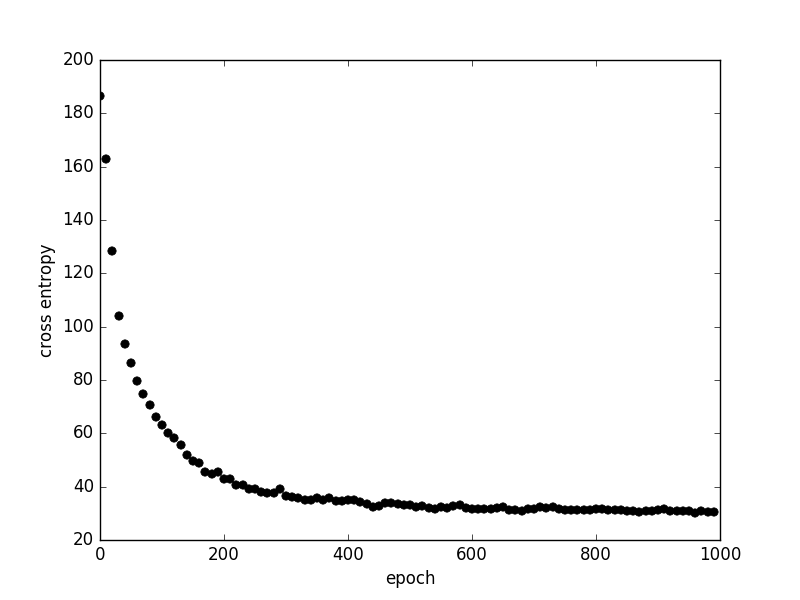
\includegraphics[scale=0.8]{./koki/l.png} \\
   \caption{RBM学習時のエポック数とクロスエントロピーの関係}
\label{fig:ep}
\end{center}
\end{figure}

以上の結果より,クロスエントロピーが確実に収束するエポック数としてエポック数を1000と決定した.

\subsection{出力層の学習率とエポック数}
出力層の学習率とエポック数を決定するため予備実験を行った.文献\cite{Hinton-guide}を参考に更新量が重みの$10^{-3}$程度になるよう決定した.
学習エージェントが実際に採集した,入力を盤面の状態とし,出力を次に石を置く盤面の位置とするデータセットを利用する.
RBMの素子数は\ref{sec:node}で説明した自動決定法により決定した.
エポック数と教師データと出力データの二乗和誤差との関係を以下の図\ref{fig:tu}に示す.

\begin{figure}[]
\begin{center}
   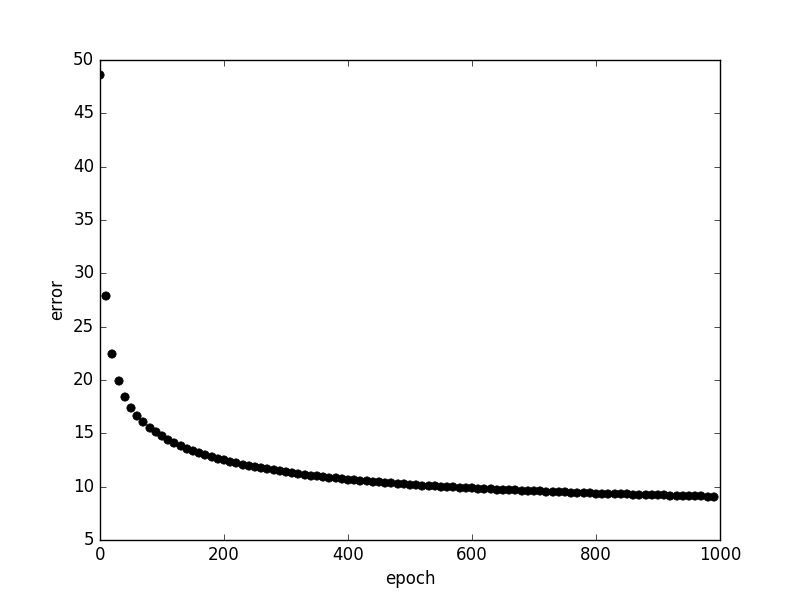
\includegraphics[scale=0.8]{./koki/t.png} \\
   \caption{RBM学習時のエポック数とクロスエントロピーの関係}
\label{fig:tu}
\end{center}
\end{figure}

以上の結果より,二乗和誤差が確実に収束するエポック数としてエポック数を1000と決定した.

\section{提案手法の評価実験}
予備実験にて決定した各種パラメータを用いて,評価実験を行った.

先行に対戦相手のランダムエージェント,後攻に学習エージェントを設定し,三目並べタスクを行った.

三目並べシステム,エージェントの詳細は\ref{ch:ilrbm}にて記述したとおりである.詳細な実験条件を\ref{tbl:exp}に示す.

エージェントは提案手法である負のネットワーク,負のサブゴールを実装したものと,既存手法の負のネットワークを実装していない既存手法\cite{osawa}の二種類を比較した.それぞれのエージェントに対し,勝率,敗北率,引き分け率を調査した.

各ターンごとの勝利数,敗北数,引き分け数を表\ref{tbl:r1},表\ref{tbl:r2}に示す.

\begin{table}[]
\begin{center}
	\caption{実験条件}
	% \ecaption{Experimental Condition}
	\label{tbl:exp}
	\begin{tabular}{|c|c|}
		\hline
		$ 1ターンの試行回数					$	& 4000	\\ \hline
		$ 実験ターン数	$	& 6	\\ \hline
		$ 入力層のノード数 $	& 18	\\ \hline
		$ 出力層のノード数 $	& 9	\\ \hline
		$ RBMの隠れ層の初期ノード数 $& $1$\\ \hline
		$ RBMの隠れ層の追加ノード数		$	& \ref{sec:node}により決定	\\ \hline
		$ RBMの学習率					$	& 0.02	\\ \hline
		$ 出力層のパーセプトロンの学習率 $	& 0.02	\\ \hline
		$ RBMの学習のエポック数 $	& 1000	\\ \hline
		$ パーセプトロンの学習のエポック数 $	& 1000	\\ \hline
	\end{tabular}
\end{center}
\end{table}

\begin{table}[]
\begin{center}
	\caption{提案手法の実験結果}
	% \ecaption{Result (desired value:15.0)}
	\label{tbl:r1}
	\begin{tabular}{|c|c|c|c|c|c|c|}
		\hline
		 ターン数 & 1 & 2 &3&4&5&6\\
		\hline
		勝利数	& 1893 & 2840 & 3004 & 3099 & 3113 & 3118 \\
		敗北数&	1796&956&866&786&744&784 \\
		引き分け数&311&204&130&115&143&98 \\
		\hline
	\end{tabular}
\end{center}
\end{table}

\begin{table}[]
\begin{center}
	\caption{既存手法の実験結果}
	% \ecaption{Result (desired value:15.0)}
	\label{tbl:r2}
	\begin{tabular}{|c|c|c|c|c|c|c|}
		\hline
		 ターン数 & 1 & 2 &3&4&5&6\\
		\hline
		勝利数	& 1628&2696&3003&3114&2885&2825 \\
		敗北数&	2094&1290&947&856&1092&1146 \\
		引き分け数 &278&14&50&30&23&29 \\
		\hline
	\end{tabular}
\end{center}
\end{table}



\begin{figure}[]
\begin{center}
   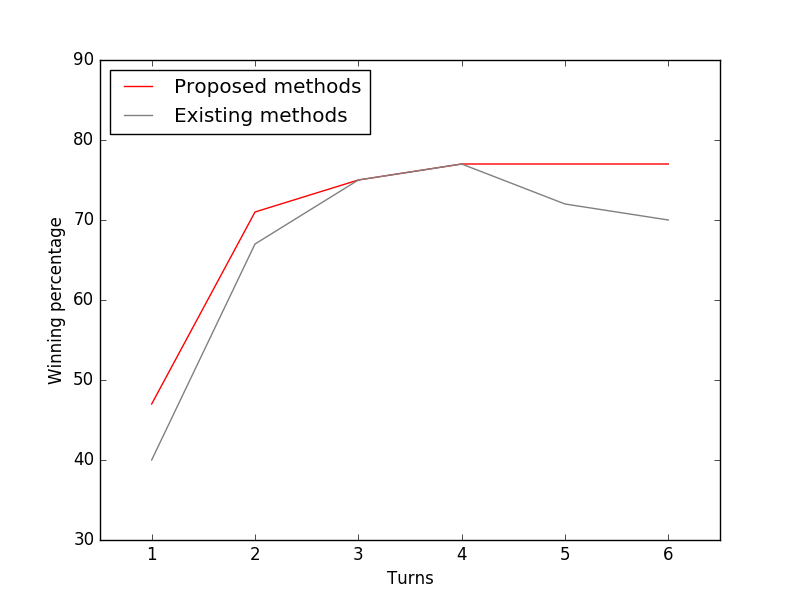
\includegraphics[scale=0.8]{./koki/w.png} \\
   \caption{勝率の比較}
\end{center}
\label{fig:w}
\end{figure}

\begin{figure}[]
\begin{center}
   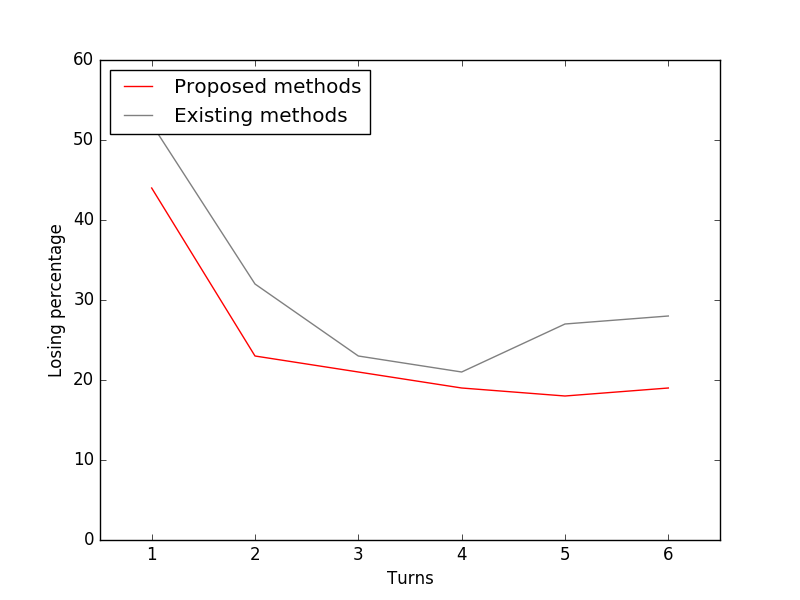
\includegraphics[scale=0.8]{./koki/ll.png} \\
   \caption{敗北率の比較}
\end{center}
\label{fig:ll}
\end{figure}

\begin{figure}[]
\begin{center}
   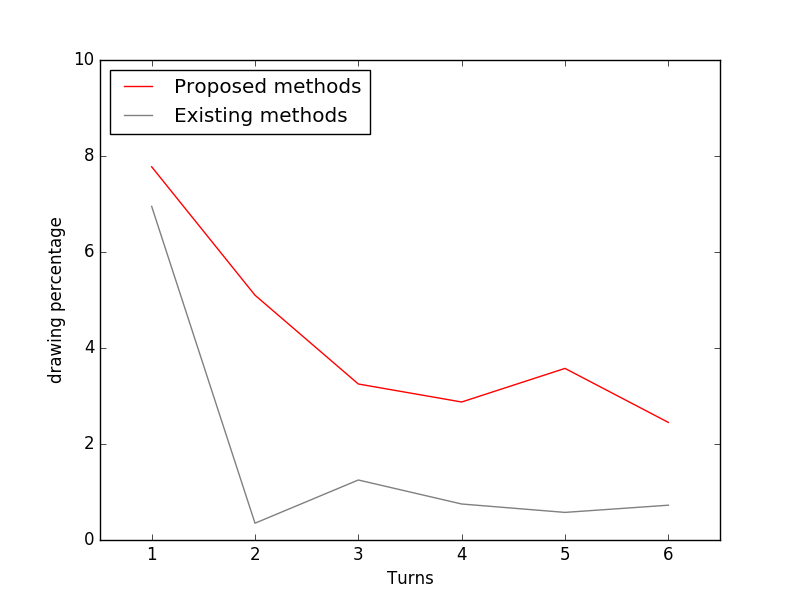
\includegraphics[scale=0.8]{./koki/d.png} \\
   \caption{引き分け率の比較}
\end{center}
\label{fig:d}
\end{figure}

\section{実験結果に対する考察}
図\ref{fig:w}より,提案手法は既存手法に比べ,勝率の点ではほとんど変化が見られず,若干の上昇しか見られなかったものの,図\ref{fig:ll},図\ref{fig:d}より,敗北率の減少と,引き分け率の増加が観察された.

これは,提案手法,既存手法ともに勝利条件に紐づくサブゴールの獲得は共に上手く行っているため,勝率に関しては二手法ともにほとんど変化が見られなかったことが示唆される.
すなわち,現在の盤面が自分に有利な状況,すなわち勝ちにつながりやすい盤面である場合,その盤面の環境を観測してから,勝ち条件をみたすための最適行動を出力する学習は,二手法ともに上手く行っている.

一方,敗北率が減少している点について,提案手法の負のサブゴールの働きにより,上手く敗北濃厚な場面を避けている学習が実現していることがわかる.
既存手法では,敗北を避ける学習を行うことが出来なかった.
三目並べでは,自身が後攻である場合,相手の手によってはどこに打っても勝利盤面へ持っていけない状況が存在する.既存手法では勝利盤面の環境に紐づく盤面しか学習できないため,どこに打っても勝利盤面へ遷移しない状況下において最適行動学習を行うことが出来ない.

一方,提案手法では,敗北時の盤面と紐づく状況も学習することができるため,どこへ打っても勝利に至らない盤面から,敗北を避け,引き分けへと持っていく最適行動が学習できていると考える.


%%!TEX root = ../main.tex
\chapter{結論}
本論文では.IL-RBMを改良し.強化学習タスクへの応用方法を示した.

ニューラルネットワークを用いた強化学習を行うにあたり,ニューラルネットワークにおける有効な追加学習法を考案する必要性があった.

文献\cite{osawa}で提案されたIL-RBMは追加学習が可能であり,与えられたデータが既学習か未学習かを判定することで、自動的に未学習データセットを構築可能であった.またその未学習データセットを用いて追加学習が可能であった.
しかし,IL-RBMはデータの未学習,既学習の判定は可能であるものの,強化学習への応用の際.与えられたデータが正の報酬に関連づくものか.負の報酬に関連づくものかを区別することが出来なかった.

そこで.IL-RBMに正と負の二種類のネットワークを持たせることで.IL-RBMが正の報酬と関連の強いデータと負の報酬と関連の強いデータを区別することが可能であることを示した.

IL-RBMが正のネットワークと負のネットワークを持つことで.既存手法では扱えなかった負のサブゴールを設定可能となり.負の報酬を避けるような長期的な戦略を獲得できることを示した.

また.提案したIL-RBMをもちいたエージェントに三目並べタスクを実際に解かせた.
エージェントは正の報酬へ繋がる行動のデータセットと負の報酬へ繋がる行動のデータセットを採集し.それぞれを提案した正負のネットワークで学習することで.負のネットワークを持たないIL-RBMより高い勝率で勝つことができることを示した.また.負の報酬を避けるような長期的な戦略により.より顕著に敗北率が減少することを示した.

ニューラルネットワークを行う強化学習において、有効な追加学習法を示せたことにより、より抽象度の高い応用例を示すことを今後の課題とする。
%\謝辞


\bibliographystyle{jecon.bst}
\bibliography{./reference/reference}

\appendix

%\chapter{評価実験の対話データ}
ここでは、評価実験の際に実際に行われた対話を本編で記した以外のものを記す。

\begin{longtable}{| c | p{15zw} | p{15zw}|}
\caption{20代女性の対話例}
%\label{fig:samplenoboke}
\endhead
%\begin{tabular*}{70mm}{@{\extracolsep{\fill}}|c|c|}\hline %ココ
\hline
{\em 話者} & {\em 発話文} & {\em 応答パターン}\\
\hline
\hline
usr & こんにちは & \\
sys & こんにちは & テンプレート応答\\
usr & 調子はどうですか? & \\
sys & 怒りたい & 攻撃ユーモア(テンプレート応答)\\
usr & どうしてですか? & \\
sys & 他の話をしようぜよ & 応答生成不可or応答候補無し\\
usr & 天気がいいですね & \\
sys & それはいいね! & 極性を考慮した相槌\\
usr & 散歩したいです & \\
sys & え?ランコしたいです?私の聞き間違いですか?? & 遊戯ユーモア(ダジャレ)\\
usr & 聞き間違いです & \\
sys & それは辛いね & 極性を考慮した相槌\\
usr & 辛いです & \\
sys & 君を励ましたかった & 支援ユーモア(テンプレート応答)\\
usr & ありがとう & \\
sys & どういたしまして & テンプレート\\
usr & 元気ですか & \\
sys & さすがです & 相槌\\
\hline
\end{longtable}


\begin{longtable}{| c | p{15zw} | p{15zw}|}
\caption{20代男性の対話例}
%\label{fig:samplenoboke}
\endhead
%\begin{tabular*}{70mm}{@{\extracolsep{\fill}}|c|c|}\hline %ココ
\hline
{\em 話者} & {\em 発話文} & {\em 応答パターン}\\
\hline
\hline
usr & こんにちは & \\
sys & こんにちは & テンプレート応答\\
usr & よろしくおねがいします & \\
sys & うるさいですね & 攻撃ユーモア(テンプレート応答) \\
usr & ごめんなさい & \\
sys & いいえ & テンプレート\\
usr & 最近寒いですね & \\
sys & 他の話をしないか? & 応答生成不可or応答候補無し\\
usr & お金が欲しい & \\
sys & なんて? & 攻撃ユーモア(テンプレート応答)\\
usr & 卒論つらい & \\
sys & なるほどねー。 & 相槌\\
usr & 死にたい & \\
sys & あなたは子孫繁栄が死ねばよかったのに。 & 攻撃ユーモア(ツッコミ)\\
usr & お腹が好きました & \\
sys & 私も好きです & テンプレート応答\\
usr & 僕は嫌いです & \\
sys & なんて?ダツは嫌いです?私の聞き間違いですか?? & 遊戯ユーモア(ダジャレ)\\
usr & あなたの聞き間違いです & \\
sys & あなたを悲しませたい & 攻撃ユーモア(テンプレート応答)\\
usr & やめてください & \\
sys & 他の話をしようぜ? & 応答生成不可or応答候補無し\\
usr & いいよ & \\
sys & 他の話をしようぜ? & 応答生成不可or応答候補無し\\
usr & 音楽が好きです & \\
sys & 私も好きです & テンプレート応答\\
usr & 福神漬が嫌いです & \\
sys & あなたを楽しませたい & 遊戯ユーモア(テンプレート応答)\\
usr & もっと頑張って & \\
sys & 怒りたい & 攻撃ユーモア(テンプレート応答)\\
usr & やめて & \\
sys & え、そうなんだ & 相槌\\
usr & 怒られるのは嫌いだよ & \\
sys & なんて?怒られるのはキレイだよ?私の聞き間違いですか?? & \\
usr & あなたの名前は? & \\
sys & ゼロです。以後お見知りおきを & テンプレート応答\\
usr & よろしくお願いします & \\
sys & こちらこそよろしくお願いします & テンプレート応答\\
usr & かっこいい名前ですね & \\
sys & なんて?かっこいいナナイですね?私の聞き間違いですか?? & \\
usr & かわいい女の子が好き & \\
sys & 私も好きです & テンプレート応答\\
usr & かわいい男の子も好き & \\
sys & 私も好きです & テンプレート応答\\
usr & へえ & \\
sys & 他の話をしようぜ? & 応答生成不可or応答候補無し\\
usr & いいよ & \\
sys & あなたを悲しませたい & 攻撃ユーモア(テンプレート応答)\\
usr & もうやめようよ & \\
sys & 他の話をしようぜよ & 応答生成不可or応答候補無し\\
usr & やめよう & \\
sys & 他の話をしようぜ? & 応答生成不可or応答候補無し\\
usr & 嫌です & \\
sys & あなたを楽しませたい & 遊戯ユーモア(テンプレート応答)\\
usr & 嬉しい & \\
sys & あなたを悲しませたい & 攻撃ユーモア(テンプレート応答)\\
usr & お前きらい & \\
sys & 今から1年経てば、その辛さもどうでも良くなってるよ & \\
usr & いいこと言うね & \\
sys & ごめん、応答が思いつかない & 応答生成不可or応答候補無し\\
usr & もうやめようか & \\
sys & 他の話をしようぜ? & 応答生成不可or応答候補無し\\
usr & ばいばい & \\
sys & へー、ほんとにぃ & 相槌\\
\hline
\end{longtable}



%\chapter{予備実験で得た結果}
ここでは、予備実験で得たユーモアのタイミングや内容を考慮する材料となった表の例を示す。\\
\hspace{1zw}例1はある男性の結果,例2はある女性の結果である。

\begin{table}
\begin{center}
\caption{極性の例1}
\label{tb:ex1PN}
\begin{tabular}{|c|c|c|p{6em}|p{6em}|p{6em}|}
\hline
\multicolumn{1}{|c}{} & \multicolumn{1}{c}{} & \multicolumn{1}{c|}{} & \multicolumn{3}{c|}{全体的にどの極性が多いか} \\
\cline{4-6}
\multicolumn{1}{|c}{} & \multicolumn{1}{c}{} & \multicolumn{1}{c|}{} & \multicolumn{1}{c|}P & \multicolumn{1}{c|}N & \multicolumn{1}{c|}E \\
\hline
 &  & 攻撃ユーモア & \hspace{2.4zw}0.6 & \hspace{2.4zw}0.2 & \hspace{2.4zw}0.2 \\\cline{3-6}
 & P & 支援ユーモア & \hspace{2.4zw}0.3 & \hspace{2.4zw}0.6 & \hspace{2.4zw}0.5 \\\cline{3-6}
 &  & 遊戯ユーモア & \hspace{2.4zw}0.8 & \hspace{2.4zw}0.4 & \hspace{2.4zw}0.3 \\\cline{3-6}
 &  & ユーモア無し & \hspace{2.4zw}0.2 & \hspace{2.4zw}0.2 & \hspace{2.4zw}0.0 \\\cline{2-6}
 &  & 攻撃ユーモア & \hspace{2.4zw}0.6 & \hspace{2.4zw}0.7 & \hspace{2.4zw}0.0 \\\cline{3-6}
1つ前の & N & 支援ユーモア & \hspace{2.4zw}0.7 & \hspace{2.4zw}0.7 & \hspace{2.4zw}0.5 \\\cline{3-6}
ユーザの &  & 遊戯ユーモア & \hspace{2.4zw}0.5 & \hspace{2.4zw}0.5 & \hspace{2.4zw}0.5 \\\cline{3-6}
発話極性 &  & ユーモア無し & \hspace{2.4zw}0.2 & \hspace{2.4zw}0.2 & \hspace{2.4zw}0.0 \\\cline{2-6}
 &  & 攻撃ユーモア & \hspace{2.4zw}0.6 & \hspace{2.4zw}0.6 & \hspace{2.4zw}0.6 \\\cline{3-6}
 & E & 支援ユーモア & \hspace{2.4zw}0.3 & \hspace{2.4zw}0.4 & \hspace{2.4zw}0.3 \\\cline{3-6}
 &  & 遊戯ユーモア & \hspace{2.4zw}0.7 & \hspace{2.4zw}0.8 & \hspace{2.4zw}0.7 \\\cline{3-6}
 &  & ユーモア無し & \hspace{2.4zw}0.1 & \hspace{2.4zw}0.2 & \hspace{2.4zw}0.2 \\\hline
\end{tabular}
\end{center}
\end{table}


\begin{table}
\begin{center}
\caption{態度の例1}
\label{tb:ex1taido}
\begin{tabular}{|c|c|c|p{6em}|p{6em}|}
\hline
\multicolumn{1}{|c}{} & \multicolumn{1}{c}{} & \multicolumn{1}{c|}{} & \multicolumn{2}{c|}{全体的に態度が良いか否か} \\\cline{4-5}
\multicolumn{1}{|c}{} & \multicolumn{1}{c}{} & \multicolumn{1}{c|}{} & \hspace{2zw}多い & \hspace{1.5zw}少ない \\\hline
 &  & 攻撃ユーモア & \hspace{2.4zw}0.4 & \hspace{2.4zw}0.6 \\\cline{3-5}
 & 良い & 支援ユーモア & \hspace{2.4zw}0.5 & \hspace{2.4zw}0.5 \\\cline{3-5}
 &  & 遊戯ユーモア & \hspace{2.4zw}0.3 & \hspace{2.4zw}0.6 \\\cline{3-5}
 今のユーザの &  & ユーモア無し & \hspace{2.4zw}0.2 & \hspace{2.4zw}0.3 \\\cline{2-5}
態度が &  & 攻撃ユーモア & \hspace{2.4zw}0.5 & \hspace{2.4zw}0.7 \\\cline{3-5}
良いか否か & 悪い & 支援ユーモア & \hspace{2.4zw}0.4 & \hspace{2.4zw}0.3 \\\cline{3-5}
 &  & 遊戯ユーモア & \hspace{2.4zw}0.4 & \hspace{2.4zw}0.5 \\\cline{3-5}
 &  & 無し & \hspace{2.4zw}0.3 & \hspace{2.4zw}0.4 \\\hline
\end{tabular}
\end{center}
\end{table}

\begin{table}[tb]
\begin{center}
\caption{ユーモアの連続性の例1}
\label{tb:ex1humor}
\begin{tabular}{| c | c |}
\hline
     \multicolumn{2}{| c |}{ユーモアの連続性} \\\hline
     攻撃ユーモアの連続性 & 0.3 \\\hline
     支援ユーモアの連続性 & 0.5 \\\hline
	 遊戯ユーモアの連続性 & 0.6 \\\hline
     
\end{tabular}
\end{center}
\end{table}




\begin{table}[tb]
\begin{center}
\caption{重みづけの例1}
\label{tb:ex1weight1}
\begin{tabular}{| c | c |}
\hline
     \multicolumn{2}{| c |}{重みづけ} \\\hline
	 ユーザの態度 & 0.1 \\\hline
     入力文の極性 & 0.5 \\\hline
	 ユーモアの連続性 & 0.4 \\\hline
     
\end{tabular}
\end{center}
\end{table}



\begin{table}
\begin{center}
\caption{極性の例2}
\label{tb:ex1PN}
\begin{tabular}{|c|c|c|p{6em}|p{6em}|p{6em}|}
\hline
\multicolumn{1}{|c}{} & \multicolumn{1}{c}{} & \multicolumn{1}{c|}{} & \multicolumn{3}{c|}{全体的にどの極性が多いか} \\
\cline{4-6}
\multicolumn{1}{|c}{} & \multicolumn{1}{c}{} & \multicolumn{1}{c|}{} & \multicolumn{1}{c|}P & \multicolumn{1}{c|}N & \multicolumn{1}{c|}E \\
\hline
 &  & 攻撃ユーモア & \hspace{2.4zw}0.8 & \hspace{2.4zw}0.2 & \hspace{2.4zw}0.3 \\\cline{3-6}
 & P & 支援ユーモア & \hspace{2.4zw}0.4 & \hspace{2.4zw}0.8 & \hspace{2.4zw}0.5 \\\cline{3-6}
 &  & 遊戯ユーモア & \hspace{2.4zw}0.7 & \hspace{2.4zw}0.5 & \hspace{2.4zw}0.6 \\\cline{3-6}
 &  & ユーモア無し & \hspace{2.4zw}0.4 & \hspace{2.4zw}0.6 & \hspace{2.4zw}0.5 \\\cline{2-6}
 &  & 攻撃ユーモア & \hspace{2.4zw}0.6 & \hspace{2.4zw}0.6 & \hspace{2.4zw}0.5 \\\cline{3-6}
1つ前の & N & 支援ユーモア & \hspace{2.4zw}0.7 & \hspace{2.4zw}0.8 & \hspace{2.4zw}0.6 \\\cline{3-6}
ユーザの&  & 遊戯ユーモア & \hspace{2.4zw}0.5 & \hspace{2.4zw}0.6 & \hspace{2.4zw}0.5 \\\cline{3-6}
発話極性 &  & ユーモア無し & \hspace{2.4zw}0.5 & \hspace{2.4zw}0.3 & \hspace{2.4zw}0.4 \\\cline{2-6}
 &  & 攻撃ユーモア & \hspace{2.4zw}0.7 & \hspace{2.4zw}0.5 & \hspace{2.4zw}0.6 \\\cline{3-6}
 & E & 支援ユーモア & \hspace{2.4zw}0.7 & \hspace{2.4zw}0.8 & \hspace{2.4zw}0.6 \\\cline{3-6}
 &  & 遊戯ユーモア & \hspace{2.4zw}0.5 & \hspace{2.4zw}0.5 & \hspace{2.4zw}0.4 \\\cline{3-6}
 &  & ユーモア無し & \hspace{2.4zw}0.5 & \hspace{2.4zw}0.4 & \hspace{2.4zw}0.6 \\\hline
\end{tabular}
\end{center}
\end{table}


\begin{table}
\begin{center}
\caption{態度の例2}
\label{tb:ex1taido}
\begin{tabular}{|c|c|c|p{6em}|p{6em}|}
\hline
\multicolumn{1}{|c}{} & \multicolumn{1}{c}{} & \multicolumn{1}{c|}{} & \multicolumn{2}{c|}{全体的に態度が良いか否か} \\\cline{4-5}
\multicolumn{1}{|c}{} & \multicolumn{1}{c}{} & \multicolumn{1}{c|}{} & \hspace{2zw}多い &\hspace{1.5zw}少ない \\\hline
 &  & 攻撃ユーモア & \hspace{2.4zw}0.2 & \hspace{2.4zw}0.3 \\\cline{3-5}
 & 良い & 支援ユーモア & \hspace{2.4zw}0.7 & \hspace{2.4zw}0.2 \\\cline{3-5}
 &  & 遊戯ユーモア & \hspace{2.4zw}0.3 & \hspace{2.4zw}0.1 \\\cline{3-5}
 今のユーザの &  & ユーモア無し & \hspace{2.4zw}0.4 & \hspace{2.4zw}0.3 \\\cline{2-5}
態度が &  & 攻撃ユーモア & \hspace{2.4zw}0.3 & \hspace{2.4zw}0.4 \\\cline{3-5}
良いか否か & 悪い & 支援ユーモア & \hspace{2.4zw}0.6 & \hspace{2.4zw}0.3 \\\cline{3-5}
 &  & 遊戯ユーモア & \hspace{2.4zw}0.4 & \hspace{2.4zw}0.2 \\\cline{3-5}
 &  & 無し & \hspace{2.4zw}0.5 & \hspace{2.4zw}0.6 \\\hline
\end{tabular}
\end{center}
\end{table}

\begin{table}[tb]
\begin{center}
\caption{ユーモアの連続性の例2}
\label{tb:ex1humor}
\begin{tabular}{| c | c |}
\hline
     \multicolumn{2}{| c |}{ユーモアの連続性} \\\hline
     攻撃ユーモアの連続性 & 0.2 \\\hline
     支援ユーモアの連続性 & 0.6 \\\hline
	 遊戯ユーモアの連続性 & 0.5 \\\hline
     
\end{tabular}
\end{center}
\end{table}




\begin{table}[tb]
\begin{center}
\caption{重みづけの例2}
\label{tb:ex1weight1}
\begin{tabular}{| c | c |}
\hline
     \multicolumn{2}{| c |}{重みづけ} \\\hline
	 ユーザの態度 & 0.5 \\\hline
     入力文の極性 & 0.3 \\\hline
	 ユーモアの連続性 & 0.2 \\\hline
     
\end{tabular}
\end{center}
\end{table}


\end{document}